\chapter{Základné pojmy}
\label{kap:kapitola1} % id kapitoly pre pre prikaz ref

\section{Jednoparametrický systém}
Ak nakreslíme kružnice so stredom na x-ovej osi s polomerom 1, ako na obrázku, pohľad nám upútajú horizontálne priamky $y = \pm 1$ idúce ponad a popod systém kružníc.

\begin{figure}[h]
	\centering
	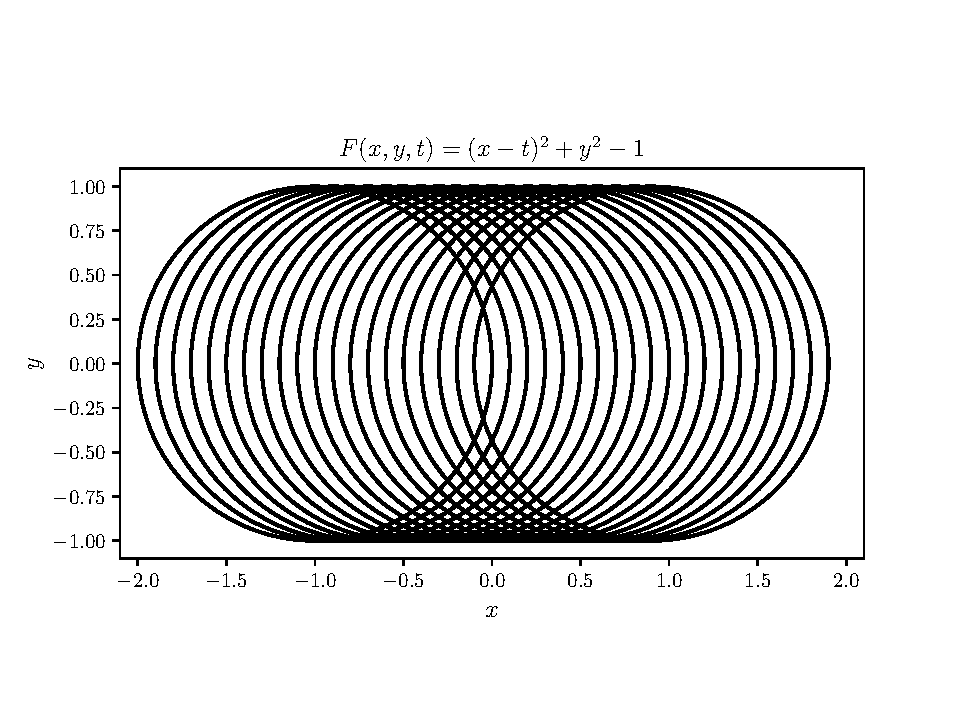
\includegraphics{images/system.pdf}
	\caption[Systém kružníc.]{Systém kružníc.}
	\label{fig:system}
\end{figure}

Každá z týchto priamok sa dotýka každej kružnice v jednom bode a v tomto bode majú spoločnú dotyčnicu. V nasledovnom texte túto myšlienku matematicky opíšeme, na základe nej zostrojíme tzv. obálku systému kriviek alebo plôch a porovnáme prístupy ich výpočtu. Budeme pracovať v reálnom vektorovom priestore so štandardným skalárnym súčinom, teda v euklidovskom priestore, rozmeru $n = 2, 3.$ Najprv ilustrujeme príklady obálok a ich výpočet pre $ n = 2.$ Po celý čas predpokladáme, že všetky zobrazenia sú dostatočne veľakrát diferencovateľné. Tučným písmom značíme vektorovú funkciu a parametre pre prehľadnosť zápisov vynechávame, ak sú z kontextu zrejmé.

Vo všeobecnosti, začneme v $\mathbb{R}^2$ s jednoparametrickým systémom kriviek daným funkciou, v $\mathbb{R}^3$ máme jednoparametrický systém plôch.

\begin{definition}
Nech $F \colon \mathbb{R}^{n} \times I \rightarrow \mathbb{R}$ je funkcia v premenných $ x_{1}, x_{2}, \ldots, x_{n} $ a v parametri $t$, kde $I \subseteq \mathbb{R}$ je interval. Definujeme jednoparametrický systém nadplôch ako systém množín 
$$
\mathcal{F}_{t} = \{ (x_{1}, x_{2}, \ldots, x_{n}) \in \mathbb{R}^{n}, \ F(x_{1}, x_{2}, \ldots, x_{n}, t) = 0, \ t \in I \}.
$$
\end{definition}

V $n = 2$ budeme pre lepšiu prehľadnosť značiť premenné $x_{1}, x_{2}$ ako $x, y,$ pre $n = 3$ pribudne $x_{3}$ ako $z.$

Pre horeuvedený prípad teda máme jednoparameterický systém kružníc so stredmi kružníc, ktoré ležia na úsečke parametrizovanej $(t,0)$ pre $t \in [-1,1]$ a konštantným polomerom pre každú kružnicu $r = 1$ daný implicitnou funkciou
$$ \mathcal{F}_{t} = \{ (x, y) \in \mathbb{R}^{2} \mid \ F(x, y, t) = 0, \ t \in [-1,1] \}, $$
kde
$$ F(x, y, t) = (x - t)^2 + y^2 - 1.$$

Systém budeme ilustrovať zobrazením niektorých prvkov systému pre diskrétne hodnoty parametra $t$. Pre $t = -1$ je zodpovedajúca $F_{-1} \in \mathcal{F}_{t}$  kružnica s implicitnou rovnicou
$$ F_{-1}(x, y) = F(x, y, -1) = (x + 1)^2 + y^2 - 1. $$

\begin{figure}[H]
	\centering
	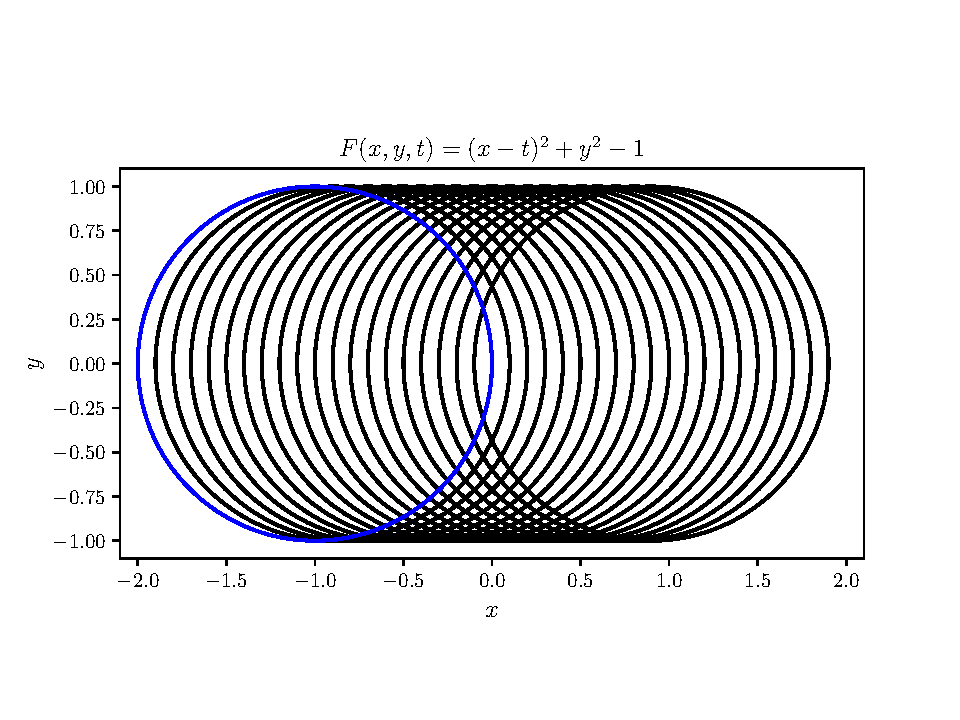
\includegraphics{images/one_element_of_system.pdf}
	\caption[Zobrazenie prvkov systému.]{Modrou farbou je vyznačená kružnica systému v parametri $t=-1$.}
	\label{fig:one_element_of_system}
\end{figure}

\section{Obálka jednoparametrického systému nadplôch}
Najskôr definujeme obálku jednoparametrického systému kriviek v $\mathbb{R}^2$. Uvedieme charakterizáciu obálok, ktorú možno použiť na výpočet pre jednoduchšie jednoparametrické systémy. Následne túto charakterizáciu použijeme ako definíciu pre obálku jednoparametrického systému plôch v $\mathbb{R}^n$.

Definujme gradient $\nabla F(x,y,t) $ vzhľadom na $x$ a $y$ ako
$$\nabla F(x, y, t) = \left(\frac{\partial F}{\partial x}(x, y, t), \frac{\partial F}{\partial y}(x, y, t) \right).$$ Predpokladáme, že $\nabla F(x,y,t) \neq \vec{0}. $ 

\begin{definition}
Obálkou systému kriviek $ \mathcal{F}_{t} $ je parametrizovaná krivka $\gamma(t) \colon J \subseteq I \rightarrow \mathbb{R}^{2}$ taká, že 
\begin{enumerate}
\item $\gamma(t) \in \mathcal{F}_{t} \text{ pre všetky } t \in J,$
\item $\dot{\gamma}(t) \perp \nabla F \left( \gamma(t), t \right).$
\end{enumerate}
\end{definition}

Obálka $\gamma(t)$ sa dotýka každej krivky zo systému $F(x,y,t)$ v bode $(x, y)$  pre nejaké $t$ a v tomto bode má s krivkou zo systému rovnakú dotyčnicu. To znamená, že každý bod obálky ${\gamma}(t) = (\gamma_{1}(t),\gamma_{2}(t))$ spĺňa rovnicu systému $F(\gamma_{1}(t),\gamma_{2}(t),t)=0$ pre nejaké $t,$ a teda platí prvá podmienka $\gamma(t) \in \mathcal{F}_{t}$. Gradient funkcie $ \nabla F(x,y,t)$ je normálový vektor k $F(x,y,t)$ v regulárnom bode $(x,y)$ a parametri $t$. V spoločnom bode $(x,y)$ a parametri $t$ chceme rovnaký smer dotykového vektora pre $\gamma(t)$ a $F(x,y,t), $ z čoho vyplýva, že $\dot{\gamma}(t)$ a dotykový vektor k funkcii $F(x,y,t)$ sú lineárne závislé, z čoho dostávame $\dot{\gamma}(t) \perp \nabla F \left( \gamma(t), t \right), $ druhú podmienku v definícii obálky. Interval $J,$ na ktorom dostávame výslednú obálku môže byť menší ako interval $I,$ na ktorom bol definovaný systém kriviek, teda máme $J \subseteq I.$ Ak by bol gradient $\nabla F(x,y,t) $ v nejakom bode nulový, nevieme nájsť jednoznačne dotykový vektor obálky a systému. 

\begin{theorem}
Regulárna krivka $\gamma(t) \colon J \subseteq I \rightarrow \mathbb{R}^{2}$ kde $t \in J  \subseteq I$ je obálkou jednoparametrického systému $\mathcal{F}_{t}$ práve vtedy, keď spĺňa:
\begin{enumerate}
\item $F(\gamma(t), t) = 0, $ 
\item $\dfrac{\partial F}{\partial t}(\gamma(t), t) = 0.$
\end{enumerate}
\end{theorem}

\begin{proof}
Táto odlišná charakterizácia je ekvivalentná definícii, ktorú sme postavili na geometrických podmienkach. Stačí zistiť korešpondenciu podmienok.
\begin{enumerate}
\item Ako sme už vysvetlili, každý bod obálky ${\gamma}(t) = (\gamma_{1}(t),\gamma_{2}(t))$ spĺňa rovnicu jednoparametrického systému $F(\gamma_{1}(t),\gamma_{2}(t),t)=0$ pre nejaké $t,$ teda podmienky 
$$ F(\gamma(t), t) = F(\gamma_{1}(t), \gamma_{2}(t), t) = 0$$
a
$$\gamma(t) \in \mathcal{F}_{t}$$
sú ekvivalentné.
\item Derivujme $F(\gamma_{1}(t),\gamma_{2}(t), t)$ podľa parametra $t,$ kde $ \dot{\gamma}(t) = ( \dot{\gamma_{1}}(t), \dot{\gamma_{2}}(t) ).$
$$ \frac{\partial F}{\partial x}(\gamma_{1}(t),\gamma_{2}(t),t) \cdot \dot{\gamma_{1}}(t)+\frac{\partial F}{\partial y}(\gamma_{1}(t),\gamma_{2}(t),t) \cdot \dot{\gamma_{2}}(t)+\frac{\partial F}{\partial t}(\gamma_{1}(t),\gamma_{2}(t),t) \cdot 1 = 0. $$
Nakoľko požadujeme, aby gradient funkcie $\nabla F(\gamma_{1}(t),\gamma_{2}(t),t)$ bol kolmý na $\dot{\gamma}(t) \text{ tak}$
$$ \langle \nabla F(\gamma_{1}(t),\gamma_{2}(t),t), \dot{\gamma}(t) \rangle = 0,$$
teda platí
$$ \frac{\partial F}{\partial x}(\gamma_{1}(t),\gamma_{2}(t),t) \cdot \dot{\gamma_{1}}(t)+\frac{\partial F}{\partial y}(\gamma_{1}(t),\gamma_{2}(t),t) \cdot \dot{\gamma_{2}}(t) = 0, $$
z čoho dostávame
$$ \frac{\partial F}{\partial t}(\gamma_{1}(t),\gamma_{2}(t),t) = 0. $$ 
\end{enumerate}
\end{proof}

Obálka sa počíta riešením rovníc
\begin{align*}
F(x, y, t) &= 0, \\
\frac{\partial F}{\partial t}(x,y,t) &= 0. \\
\end{align*}

Často sa v literatúre môžeme stretnúť s rôznymi opismi obálky, ktoré však bez ďalších predpokladov nemusia definovať rovnakú množinu bodov. Príkladom je ďalšia charakterizácia obálky ako množiny limitných bodov prienikov kriviek systému. Vzťahy medzi jednotlivými charakterizáciami možno nájsť v \cite{Bru81}.  

Dokonca, daný systém nemusí mať obálku. Príkladom sú sústredné kružnice s rastúcim polomerom.

\begin{example} 
Obálku systému sústredných kružníc pre $t \in I=[\frac{1}{10},2]$ rátame ako systém rovníc
\begin{align*}
F(x, y, t) &= x^2 + y^2 - t, \\
\frac{\partial F}{\partial t}(x,y,t) &= -1. \\
\end{align*}
Z druhej rovnice máme $t=-1 \neq 0,$ teda systém nemá riešenie. Aj keď by sa nám mohlo zdať, že by obálkou mohli byť body kružnice s najväčším polomerom $F_2$ a kružnice s najmenším polomerom $F_{\frac{1}{10}}$, práve podmienka existencie takej krivky $\gamma(t),$ ktorá by patrila do systému kružníc $\mathcal{F}_t$ pre všetky $t$ z intervalu $J \subseteq  I $ nie je splnená.
\end{example}

\begin{figure}[H]
	\centering
	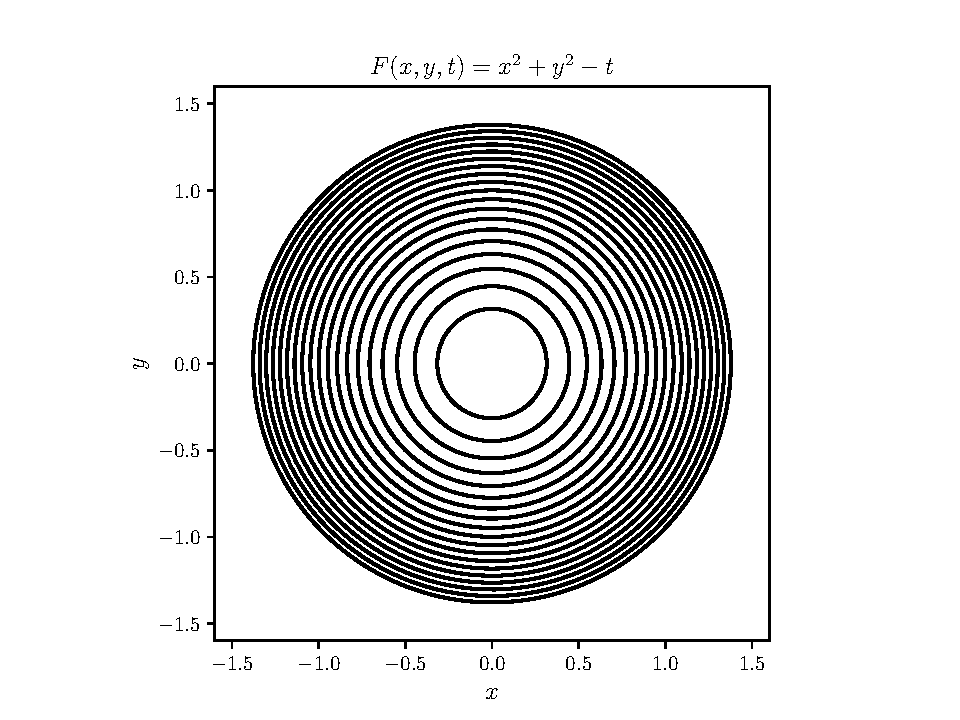
\includegraphics{images/concentric_circles.pdf}
	\caption{Sústredné kružnice.}
	\label{fig:concentric_circles}
\end{figure}


Prístup, ktorý sme využili pre jednoparametrický systém kriviek, možno zovšeobecniť pre ľubovoľný jednoparametrický systém plôch v $\mathbb{R}^n.$

\begin{definition}{\textbf{\textup{(Charakterizácia.)}}}
Obálkou jednoparametrického systému plôch $ \mathcal{F}_{t} $ je množina bodov $\mathcal{E}$ daná
$$\mathcal{E} = \{(x_{1}, x_{2}, \dots, x_{n})  \in \mathbb{R}^{n} \colon \exists t \in \mathbb{R}, F(x_{1}, x_{2}, \dots, x_{n}, t) = \frac{\partial F}{\partial t}(x_{1}, x_{2}, \dots, x_{n}, t) = 0 \}.$$
\end{definition}

Ak by sme chápali obálku podľa definície ako množinu bodov, problém by sme mohli riešiť ako systém nelineárnych rovníc v parametri $t,$ kde chceme z rovníc 
\begin{align*}
F(x,y,t) &= 0, \\
\frac{\partial F}{\partial t}(x, y, t) &= 0. \\
\end{align*}
eliminovať $t.$ Na riešenie nelineárneho systému dvoch rovníc síce existujú pokročilé nástroje, no eliminovaním parametra $t$ strácame informáciu o tom, kde je obálka definovaná. 

\begin{example}
Pre náš príklad $ F(x, y, t) = (x - t)^2 + y^2 - 1 = 0 $ máme 
$$\frac{\partial F}{\partial t}(x, y, t) = 2(t-x) = 0. $$
Ak $t = x, $ tak $y^2 = 1.$ Teda obálka je podľa tejto charakterizácie $ y = \pm 1, $ ako sme očakávali.
\end{example}

\begin{figure}[H]
	\centering
	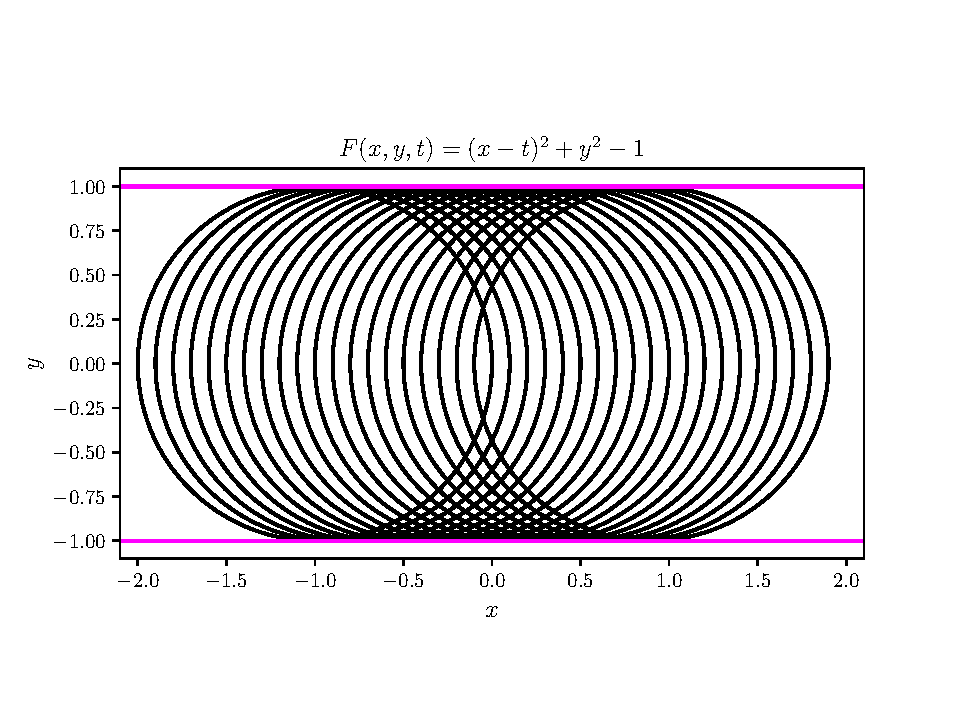
\includegraphics{images/system_with_envelope_unlimited_domain.pdf}
	\caption{Obálka systému podľa charakterizácie.}
	\label{fig:system_with_envelope_unlimited_domain}
\end{figure}

V skutočnosti sú obálkou krivky $y=\pm 1$ definované na intervale $[-1,1]$.

\begin{figure}[H]
	\centering
	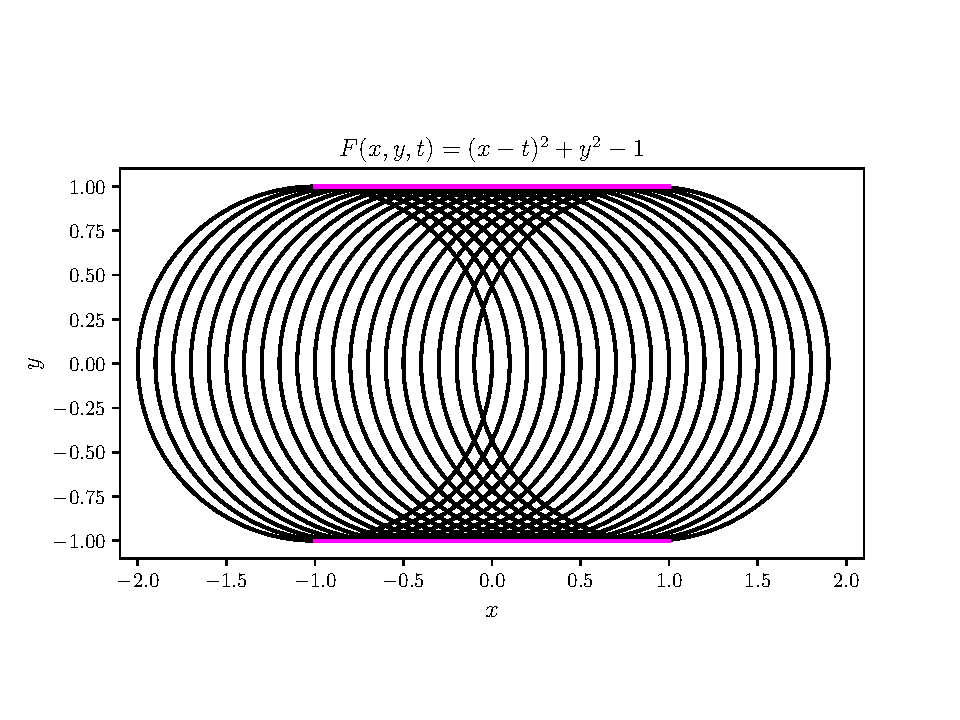
\includegraphics{images/system_with_correct_envelope.pdf}
	\caption{Obálka systému podľa definície.}
	\label{fig:system_with_correct_envelope}
\end{figure}

Tento problém možno ošetriť tak, že budeme uvažovať systémy kriviek, ktoré sú v parametri $t$ definované na celej reálnej priamke $\mathbb{R}$. 

\begin{example}
\label{example:too_complicated_equations}
Počítajme obálku systému kriviek znázornenom na obrázku \ref{fig:too_complicated_equations}, ktorý je daný
\begin{align*}
F(x,y, t) &= \dfrac{x^2}{(t^2 + 1)^2} + (y - 2t)^2 - 1, \\
\dfrac{\partial F}{\partial t}(x, y, t) &= -\dfrac{4x^2t}{\left(t^2+1\right)^3}-4\left(y-2t\right). \\
\end{align*}
Vynásobením prvej rovnice $ \lambda(t) = (t^2 + 1)^2$ a derivovaním získavame
\begin{align*}
F^\lambda &= 4 t^6 - 4 t^5 y + t^4 y^2 + 7 t^4 - 8 t^3 y + 2 t^2 y^2 + 2 t^2 - 4 t y + x^2 + y^2 - 1, \\
F_t^\lambda &= 24t^5-20yt^4+4y^2t^3+28t^3-24yt^2+4y^2t+4t-4y. \\
\end{align*}
Na obrázku \ref{fig:too_complicated_equations} je znázornený tento systém elíps. Obálku nájdeme ako riešenie $F^\lambda \cap F_t^\lambda. $ Rovnice sú však príliš vysokého stupňa v parametri $t$, preto nevieme implicitnú rovnicu obálky bez vhodného nástroja vyjadriť. V ďalšej časti rozoberieme prístupy výpočtu.
\end{example}

\begin{figure}[H]
	\centering
	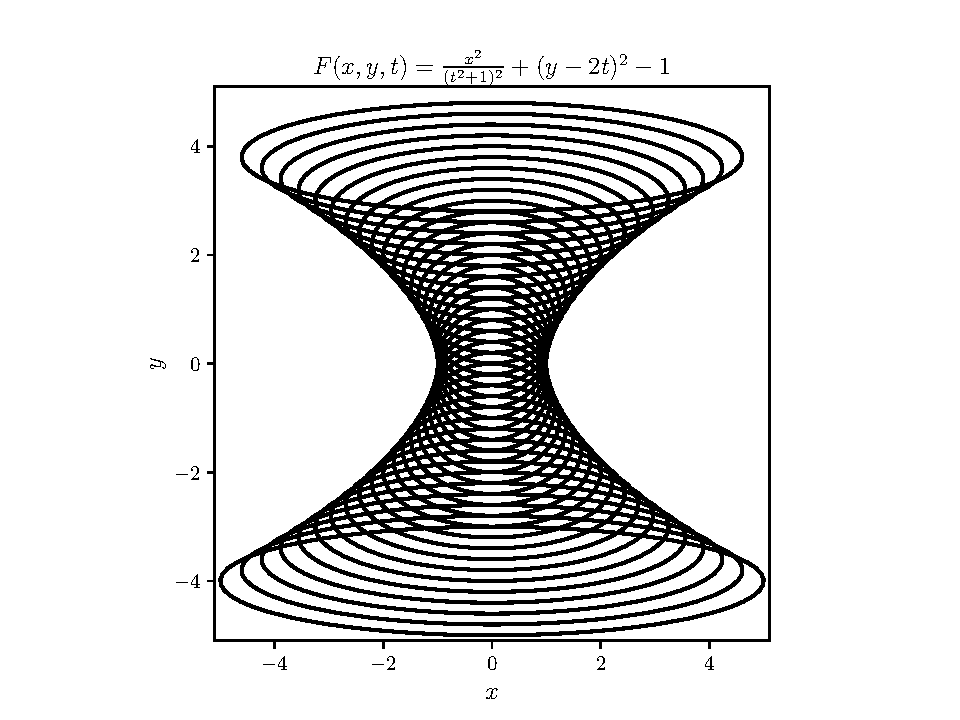
\includegraphics{images/too_complicated_equations.pdf}
	\caption{Systém elíps.}
	\label{fig:too_complicated_equations}
\end{figure}


\section{Výpočet obálky}
Vo väčšine prípadov sú rovnice charakterizujúce obálku systému plôch príliš vysokého stupňa v parametri $t$ a nedokážeme z nich ľahko odvodiť rovnicu obálky, preto pristupujeme aj k numerickým riešeniam. Spoľahlivá aproximácia obálky je jednou z aktuálnych výskumných tém. Na začiatok si však rozoberme existujúce analytické prístupy. Naledujúce prístupy sú prevzaté z \cite{Vra22}.
\subsection{Prístup algebraickej geometrie}
Dokonca aj v prípade jednoduchého príkladu ako \ref{example:too_complicated_equations}, obe polynomické rovnice charakterizujúce obálku sú vysokého stupňa v parametri $t$, preto je odstránenie parametera $t$ náročné bez vhodného nástroja. Štandardným aparátom na túto úlohu sú Gröbnerove bázy. Gröbnerove bázy sú kľúčovým pojmom v algebraickej geometrii a počítačovej algebre. Ide o špeciálnu množinu polynómov vo viacerých premenných, ktoré majú niekoľko dôležitých vlastností a zohrávajú kľúčovú úlohu pri riešení rôznych matematických problémoch vrátane riešenia sústav polynomických rovníc, zjednodušovania polynómov a dokazovania rôznych algebraických tvrdení. Vybudovanie tejto teórie je pomerne zdĺhavé, preto odkážeme na bohaté teoretické pozadie v \cite{Chalm}.
Najprv vypočítame Gröbnerovu bázu Buchbergerovým algoritmom pre ideál generovaný sústavou polynomických rovníc, ktorá obsahuje všetky premenné vrátane tej, ktorú chceme eliminovať. Z Gröbnerovej bázy vyberieme polynómy, ktoré obsahujú premennú, ktorú chceme eliminovať. Tieto polynómy použijeme na vyjadrenie tejto premennej v závislosti od ostatných premenných. Po vyriešení nových rovníc získame výraz, ktorý opisuje vzťah medzi zvyšnými premennými a eliminovanou premennou. Týmto spôsobom úspešne eliminujeme premennú.
Pokúsme sa vypočítať Gröbnerovu bázu príkladu \ref{example:too_complicated_equations} vzhľadom na lexikografické usporiadanie monómov $t > x > y $. Keďže výpočet Gröbnerovej bázy trvá pomerne dlho, neuvádzame postup a výsledok možno nájsť v prílohe \ref{pri:priloha1}.

Gröbnerova báza vzhľadom na iné usporiadanie, napr. grevlex je zvyčajne vypočítaná oveľa rýchlejšie a jej polynómy majú krajšie koeficienty, no na druhej strane, tento prístup nie je vo všeobecnosti možné použiť na odstránenie premennej $t$ z rovníc. 

Existujú aj iné metódy na riešenie polynomických rovníc, ktoré nie sú závislé na usporiadaní monómov. 
Spôsob, ako nájsť polynóm, ktorý leží v prvom eliminačnom ideáli, ktorý je nezávislý na Gröbnerovej bázach a monómických usporiadaniach, využíva teóriu rezultantov. Rezultant je determinant matice polynómov.

Hoci výpočet determinantov veľkých matíc je výpočtovo aj časovo náročný problém, existujú metódy, ako  vypočítať determinant efektívnejšie. V príklade \ref{example:too_complicated_equations} uvedieme výsledný polynóm $Res(F^\lambda , F_t^\lambda , t)$ a ukážeme obálku nájdenú rezultantom, pozri \ref{fig:resultant}. 

$ Res(F^\lambda , F_t^\lambda , t) = 191102976x^{10} + 262144x^8y^6 - 9584640x^8y^4 + 83165184x^8y^2 - 633470976x^8 - 16384x^6y^{10} - 81920x^6y^8 - 14483456x^6y^6 - 113311744x^6y^4 + 96419840x^6y^2 + 698368000x^6 - 16384x^4y^{12} - 294912x^4y^{10} - 2998272x^4y^8 - 18284544x^4y^6 - 74956800x^4y^4 - 184320000x^4y^2 - 256000000x^4. $

\begin{figure}[H]
	\centering
	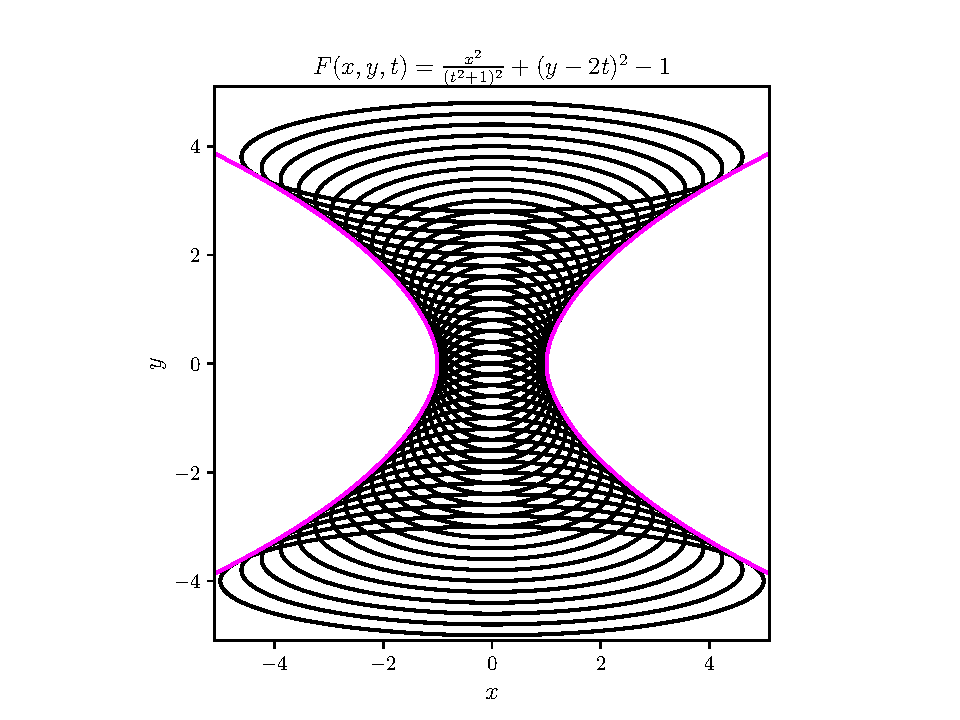
\includegraphics{images/resultant.pdf}
	\caption{Obálka vypočítaná rezultantom.}
	\label{fig:resultant}
\end{figure}

Navyše táto metóda, rovnako ako metóda založená na eliminačnej teórii s použitím Gröbnerových báz, nám vypočíta správnu obálku len vtedy, ak uvažujeme parameter $t$ jednoparametrického systému z celej reálnej priamky. Ak obmedzíme oblasť parametra na interval, tak obálka zvyčajne nemôže byť daná implicitnou rovnicou, a preto je potrebné nájsť nejakú parametrizáciu obálky. 

Pri použití rezultantov máme lepšiu kontrolu nad zložitosťou výpočtu. Pre dané dva polynómy totiž vieme, ako sa konštruuje rezultant, a tak vieme odhadnúť, s akými veľkými polynómami sa bude počas výpočtu manipulovať, avšak pri hľadaní Gröbnerovej bázy je ťažké odhadnúť, ako zložité S-polynómy sa behom algoritmu vyskytnú. Nie je zriedkavosťou, že S-polynómy sú podstatne komplikovanejšie než vstupné polynómy a výsledná Gröbnerova báza.

\subsection{Prístup projektívnej geometrie}
Pribudne neskôr.
%Body duálneho projektívneho priestoru $\mathbb{P}^3 $ možno stotožniť s nadrovinami v $\mathbb{R}^3$. Plochu v duálnom projektívnom priestore možno teda interpretovať ako množinu všetkých jej dotykových nadrovín. Duálny prístup pomôže dokázať, že obálky jednoparametrických systémov sú racionálne.

%Laguerreova geometria, cyklografické zobrazenie.

\subsection{Kinematický prístup}
Ďalším zo spôsobov, ako chápať jednoparametrické systémy plôch v $\mathbb{R}^n$ je pozerať sa na ne ako na množinu všetkých transformácií daného povrchu $P$. Povrch $P$ sa transformuje na ostatné prvky systému prostredníctvom prvkov vhodnej grupy transformácií. Táto množina transformácii má okrem štruktúry grupy aj štruktúru hladkej variety \textit{(smooth manifold)}. Tieto grupy nazývame Lieove grupy.

\begin{example}
Ilustujme tento postup na jednoduchom rovinnom príklade. Transformujme zobrazením $g_t$ priamku
\begin{align*}
l \colon x(u) &= 1 \\
y(u) &= u \\
\end{align*}
\[
g_t \begin{pmatrix} x \\ y \end{pmatrix} = \begin{pmatrix}
\cos t & -\sin t  \\
\sin t & \cos t  \\
\end{pmatrix}
\begin{pmatrix} x \\ y \end{pmatrix}.
\]
Pre každé $t \in \mathbb{R}$, $g_t$ zodpovedá rotácii. Grupa všetkých rotácií je $SO(n)$ a nazýva sa špeciálna ortogonálna grupa. Pre $t = 0$, dostávame priamku $l$. Pre iné $t$, napríklad $t = \frac{\pi}{2}$, dostávame priamku
\begin{align*}
g_t(l) \colon x(u) &= -u \\
y(u) &= 1. \\
\end{align*}
Na obrázku \ref{fig:lines_in_normal_form} je znázornená priamka $l$ modrou farbou, transformovaná priamka $g_t(l)$ červenou farbou.

\begin{figure}[H]
	\centering
	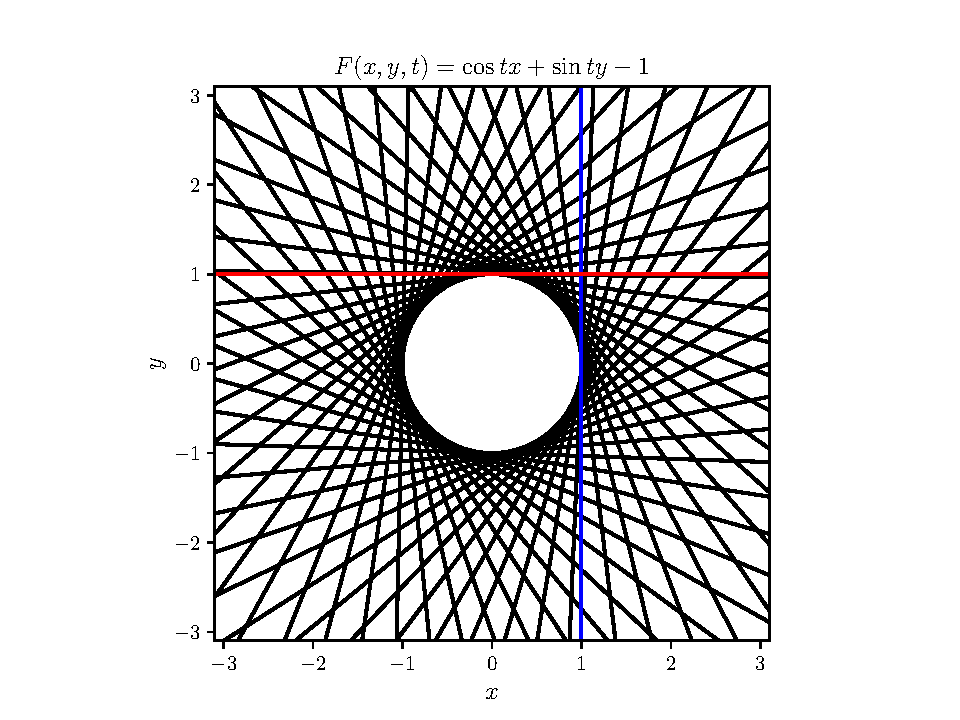
\includegraphics{images/lines_in_normal_form.pdf}
	\caption{Systém priamok v normálovom tvare.}
	\label{fig:lines_in_normal_form}
\end{figure}

\end{example}

Transformácie $g_{t}$ z príkladu sú prvkami Lieovej grupy $SO(n)$. Ďalšie známe príklady maticových Lieovych grúp sú ortogonálna grupa $O(n)$, unitárna $U(n)$ a špeciálna unitárna grupa $SU(n).$ 
Pre nájdenie podrobnejších informácií, sa môže čitateľ obrátiť na ľubovoľnú úvodnú učebnicu o Lieovych grupách a Lieovych algebrách, ako je napríklad \cite{Lee12}.
Použili sme štruktúru Lieovej grupy, aby sme opísali, ako sa grupa transformuje daný povrch. Ďalej, využijúc štruktúru hladkej variety môžeme opísať jednoparametrický systém plôch výlučne pomocou terminológie Lieových grúp. Táto teória sa aplikuje na nájdenie parametrizácie obálok kvadratických plôch. Viac o tomto prístupe možno nájsť v \cite{Vra22}. 

\subsection{Obálky a ODR}
Obálky súvisia aj so štúdiom obyčajných diferenciálnych rovníc, a najmä ich singulárnych riešení. Predpokladajme, že jednoparametrický systém kriviek $\mathcal{F}_t$ je riešením nejakej diferenciálnej rovnice prvého rádu. Potom môže existovať aj ďalšia krivka spĺňajúca túto diferenciálnu rovnicu, ktorá je dotyčnicou k $\mathcal{F}_t$ v každom bode. Táto krivka je obálka. V literatúre sa nazýva aj singulárne riešenie diferenciálnej rovnice.
Uvažujme ODR 
$$
\left(\frac{dy}{dx}\right)^2 - 4x\frac{dy}{dx} + 4y = 0.
$$
Jej regulárnym riešením sú integrálne krivky 
$$ y = - t^2 + 2tx, \text{ kde } t \in \mathbb{R}.$$
Riešenie môžeme reprezentovať ako jednoparametrický systém kriviek $\mathcal{F}_t$ s funkciou
$$F(x,y,t) = t^2 - 2tx + y. $$
Derivovaním podľa parametra $t$ dostávame
$$\dfrac{\partial F}{\partial t} (x,y,t) = 2t - 2x, $$
z čoho máme $t=x$ a dosadením do funkcie máme $F=-x^2+y,$ teda obálka je $y=x^2.$

Obálka tejto jednoparametrickej rodiny priamok, ktorou je parabola $y = x^2$, rieši taktiež diferenciálnu rovnicu. Viac o tomto prístupe možno nájsť v \cite{Gro97}.

\begin{figure}[H]
	\centering
	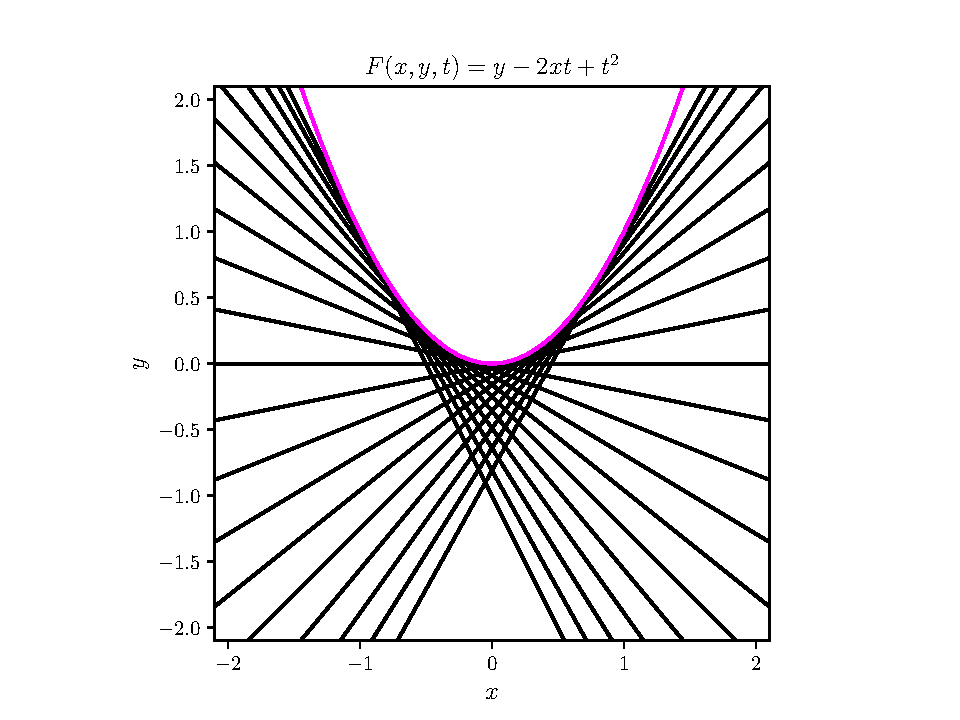
\includegraphics{images/odr.pdf}
	\caption{Regulárne riešenia a obálka.}
	\label{fig:odr}
\end{figure}

\section{Aplikácie obálok a predošlá práca}
Vzhľadom na výskyt obálok v aplikáciách sa obálkam venuje veľká pozornosť. Stručne spomenieme niektoré aplikácie a odkážeme na literatúru. 

Výpočet obálky pohybujúcej sa plochy sa vyskytuje pri simulácii a CNC obrábaní. CNC obrábanie \textit{(Computer Numerical Control machining)}  je výrobný subtraktívny proces, pri ktorom počítač riadi stroje, napríklad vŕtačky, frézy a sústruhy tak, aby neustále odlamovali obrobok. Tento postup sa vykonáva, kým sa nevytvorí požadovaný tvar. Rezný nástroj vytvára pri rýchlom otáčavom pohybe okolo svojej osi rotačnú plochu. Takto vytvorená plocha je časť obálky pohybujúceho sa nástroja. CNC frézovanie má široké priemyselné využitie v odvetviach ako letecký priemysel, zdravotníctvo a spotrebná elektronika. V článku \cite{Skop20} sa možno dočítať viac o výpočte obálok pri 5-osovom CNC obrábaní.  

Obálky sa používajú aj na výpočet trajektórie projektilu vo vzduchu. Riešime klasický problém pohybu hmotného bodu (projektilu) vrhaného pod uhlom k horizontu. S nulovou silou odporu vzduchu je analytické riešenie dobre známe, trajektória projektilu je parabola. So zohľadnením odporu vzduchu úloha nemá presné analytické riešenie, a preto sa vo väčšine prípadov rieši numericky. Silu odporu vzduchu berieme do úvahy s konštantným členom odporu. Systém trajektórií vzniká pri vrhnutí projektilu s rovnakou počiatočnou rýchlosťou, ale s rôznymi uhlami hodu. Na určenie maximálneho rozsahu letu projektilu sa tak použije rovnica obálky. \cite{Chud09}

%krivka s kontrolou chyby (Wallner)
Medzi ďalšie aplikácie obálok patrí tollerancing - krivka s kontrolou chyby, bezkolízne plánovanie pohybu robota - uvažujeme o konvexných kompaktných krivkách reprezentujúcich pohyb robota v rovine, ktorý mení svoj lokálny tvar pomocou systému afinných transformácií. Dizajn písma - konštrukcia znakov v písmach pre typografické systémy. O ďalších aplikáciach sa čitateľ dozvie v \cite{Pott09}.

Kanálové plochy \textit{(channel surfaces)}, rúrkové plochy/potrubia \textit{(pipe surfaces}), \textit{rolling ball blends} a prirodzené kanálové plochy \textit{(natural channel surfaces)} sa vyskytujú ako zmiešavacie povrchy a prechodové plochy medzi potrubiami. Kanálové plochy sú používané v počítačom podporovanom geometrickom dizajne \textit{(Computer Aided Geometric Design)}. V ďalšom texte si ukážeme ich konštrukciu ako obálku sfér.

Obálky - kanálové plochy sa využívajú aj v architektúre. Ako príklad uvádzame Webbov most \textit{(Webb Bridge)}, obr. \ref{fig:webb_bridge}, nachádzajúci sa v Melbourne v Austrálii. Tvar mosta vzdáva hold histórii domorodého obyvateľstva a je vytvorený podľa tradičnej rybárskej pasce Koorie, ktorá sa používala na lov úhorov.

\begin{figure}[h!]
	\centering
	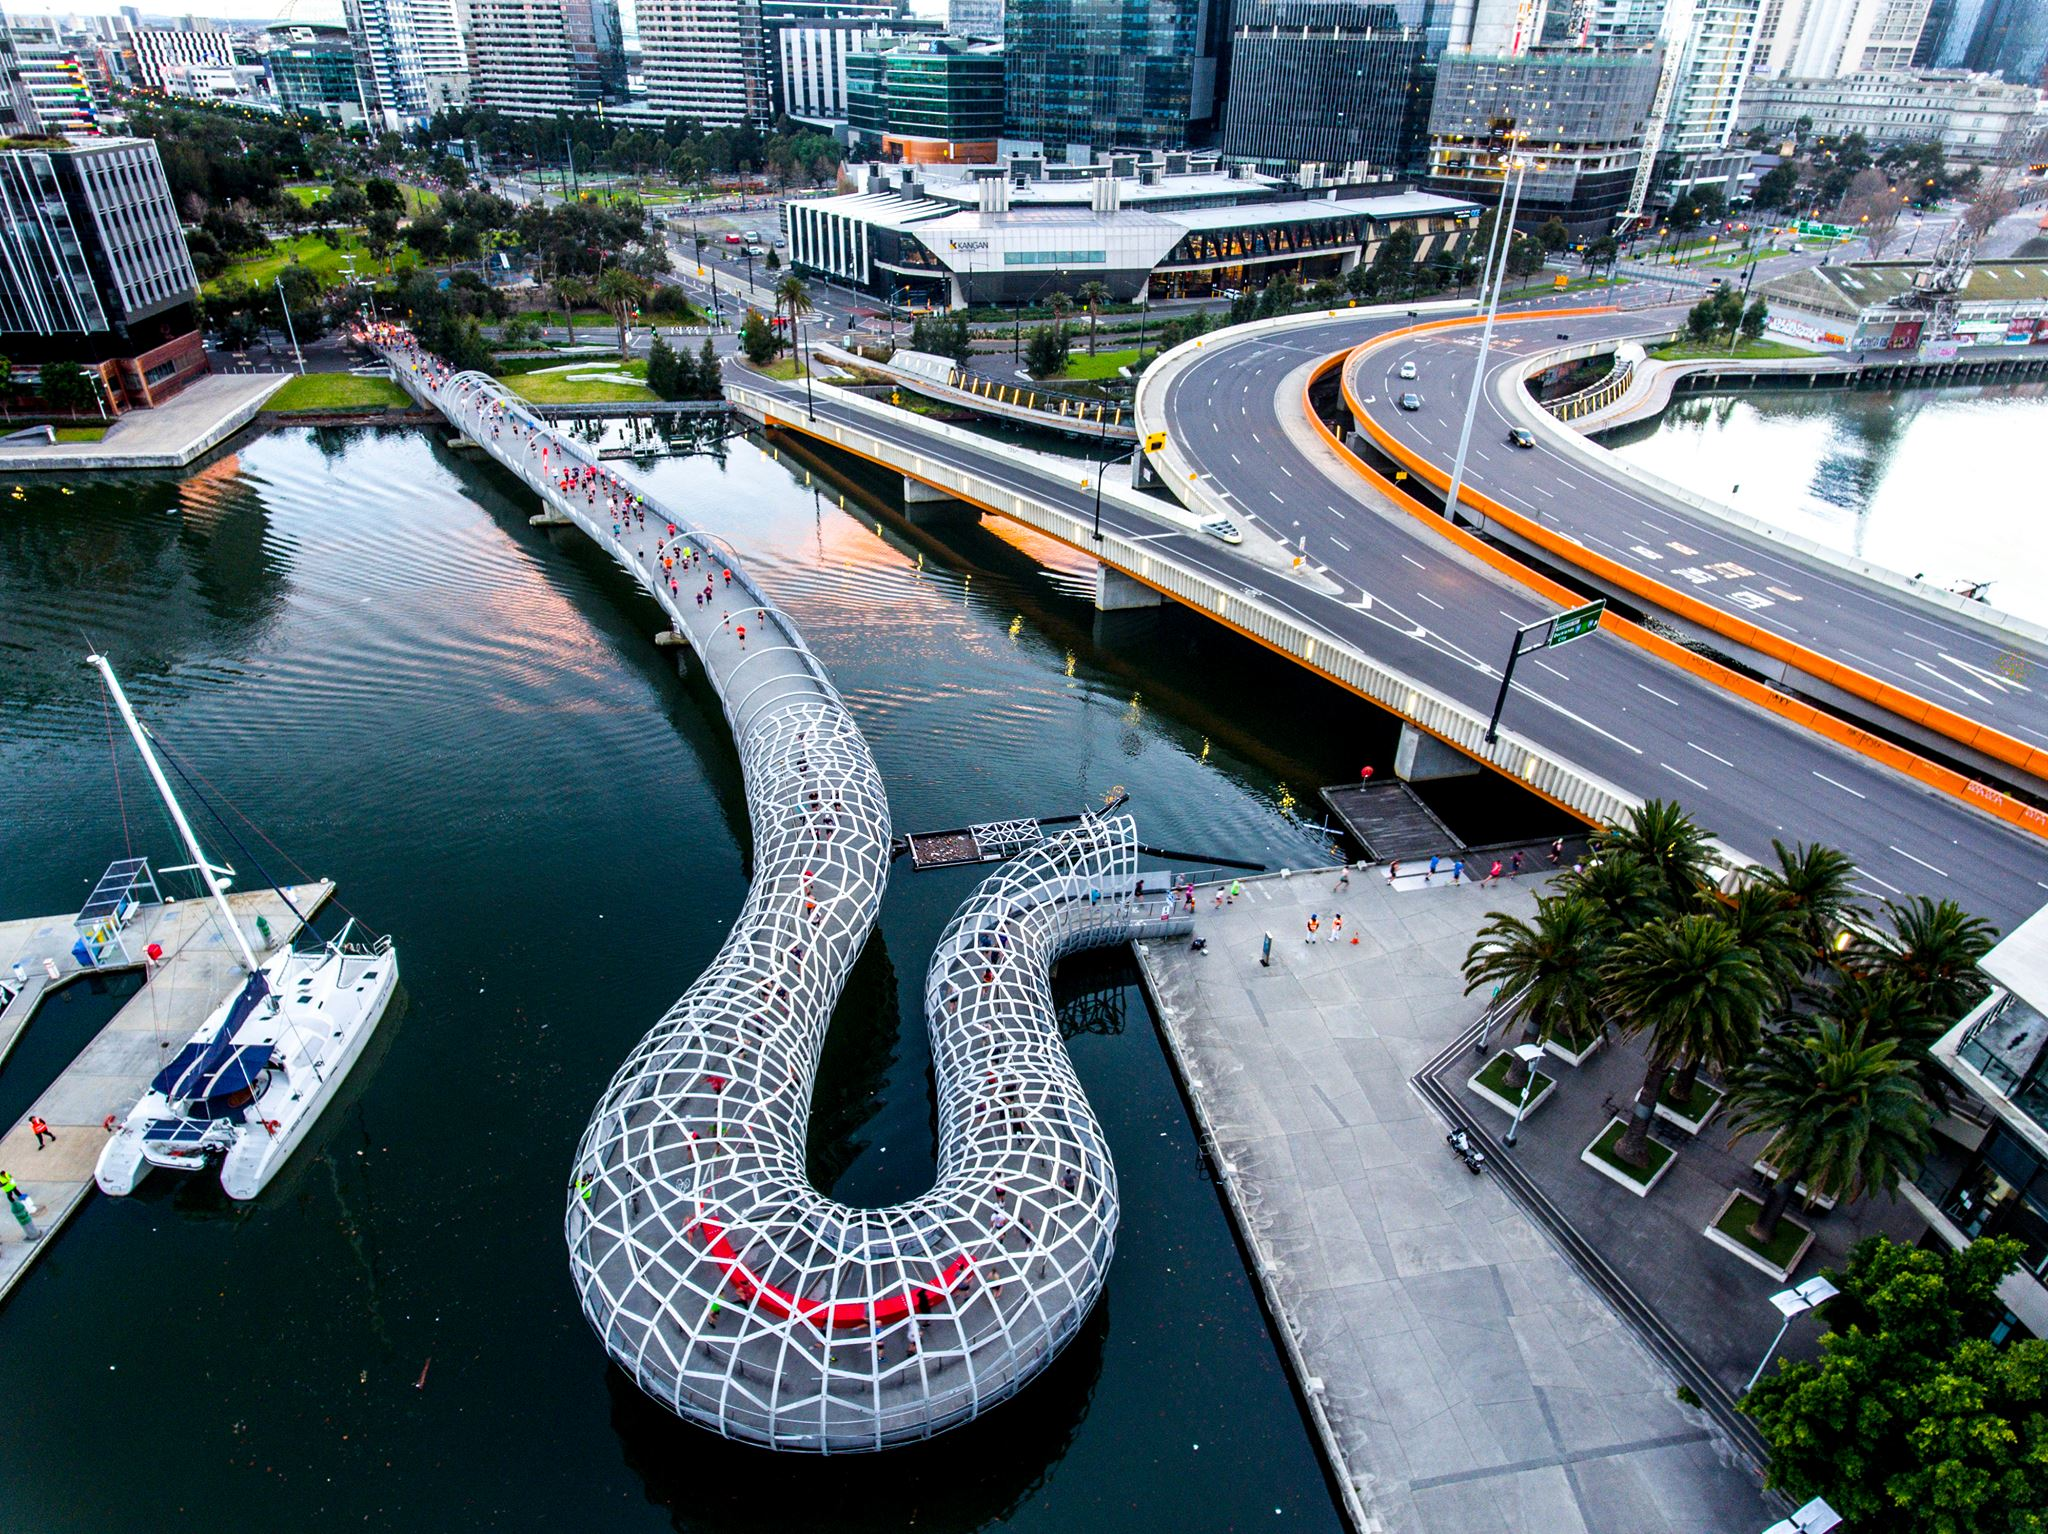
\includegraphics[width=\textwidth]{images/webb_bridge.jpg}
	\caption{Webbov most.}
	\label{fig:webb_bridge}
\end{figure}

\section{Obálka sfér}
Označme $\bold{x} = (x, y, z)$ a predpokladajme, že $\bold{m}(t) = (m_x(t), my(t), m_z(t)) \colon I \subset \mathbb{R} \rightarrow \mathbb{R}^3$ je parametrizácia krivky $\bold{m}$ a $r(t) \colon I \rightarrow \mathbb{R}^{+}$ je funkcia definovaná na tom istom intervale. Krivka $\bold{m}$ sa nazýva kostrová krivka obálky (\textit{spine curve}) a $r$ sa nazýva funkcia polomeru (\textit{radius function}). Jednoparametrický systém sfér je daný rovnicou

$$
S \colon \langle \bold{x} - \bold{m}, \bold{x} - \bold{m} \rangle - r^2(t)= 0.
$$

Podľa predchádzajúceho, obálku $\mathcal{E}$ možno nájsť ako prienik $S(t)$ a $\dot{S}(t)$ pre všetky $t \in I$. Derivácia $S$ nám dáva roviny

$$
\dot{S} \colon \langle \dot{\bold{m}}, \bold{x} - \bold{m} \rangle + r \dot{r} = 0.
$$

Z toho vyplýva, že charakteristické krivky obálky $\mathcal{E}$ pre jednoparametrický systém sfér sú kružnice. Existujú dva prípady, ktoré treba zvážiť:

Ak je funkcia polomeru $r$ konštantná, $\dot{r} \equiv 0$ a rovina $\dot{S}(t)$ obsahuje stred sféry $M$ pre všetky $t \in I$, v tomto prípade možno obálku $\mathcal{E}$ považovať za posunutie (\textit{offset}) kostrovej krivky $\bold{m}$. Tieto obálky sú známe ako rúrkové plochy (\textit{pipe surfaces}). Keďže rovina $\dot{S}$ charakteristickej kružnice $c$ obsahuje stred gule $M$ (v každom $t \in I$), charakteristická krivka je hlavnou kružnicou sféry a obálka $\mathcal{E}$ je pokrytá jednoparametrickým systémom zhodných kružníc.

Ak funkcia polomeru $r$ nie je konštantná, potom $\dot{r} \neq 0$ a rovina $\dot{S}$  neprechádza stredom sféry $M$. Prienik $S$ a $\dot{S}$ je kružnica $c$, spoločné dotyčnice roviny $S$ a obálky $\mathcal{E}$ pozdĺž $c$ tvoria rotačný kužeľ $\Gamma_{c}$. V tomto prípade obálka $\mathcal{E}$ patrí do triedy kanálových plôch. 
Stred $N$ charakteristickej kružnice $c$ nájdeme ako normálu $\bold{n}(w) = \bold{m} + w\dot{\bold{m}}$ k rovine $\dot{S},$  
teda
$$ \bold{n} = \bold{m} - \frac{r \dot{r}}{\langle \dot{\bold{m}}, \dot{\bold{m}} \rangle} \dot{\bold{m}}.$$
Charakteristická krivka má polomer
$$ r_c = \sqrt{r^2 - \|MN\|^2} = r \sqrt{ 1 - \frac{\dot{r}^2}{\langle \dot{\bold{m}}, \dot{\bold{m}} \rangle}}. $$
V prípade, že $ \|MN\| > r$, sféra $S$ nemá s obálkou $\mathcal{E}$ reálny kontakt. Vrchol $A$ dotykového kužeľa $\Gamma_c$ je pólom $\dot{S}$ vzhľadom na $S$. (tu ešte chýba výpočet vrchola)
Vrchol $A$ kužeľa je potom 
$$
A = \mathbf{m} - \frac{r} {\dot{r}}\mathbf{\dot{m}}.
$$

Jedným z dôležitých výsledkov je, že kanálové plochy, definované ako obálka jednoparametrickej množiny sfér s racionálnou funkciou polomeru $r(t)$ a stredmi v racionálnej krivke $\bold{m}(t)$ možno racionálne parametrizovať. \cite{Pet97}

\begin{example}
Uvažujme kostrovú krivku $\bold{m}(t)$ a polomer $r(t)$
$$
\bold{m}(t) = \begin{pmatrix} 0 \\ 0 \\ t \end{pmatrix} \quad \text{ a } \quad r(t) = \frac{t}{\sqrt{26}}.
$$
potom jednoparametrický systém $\mathcal{F}_t$ sfér je
$$
\mathcal{F}_t = \{(x, y, z) \in \mathbb{R}^3 \mid x^2 + y^2 + (z - t)^2 - \frac{t^2}{26} = 0, \ t \in \mathbb{R}\}.
$$
Obálka systému je daná rovnicami
\begin{align*}
&\mathcal{S} \colon x^2 + y^2 + (z - t)^2 - \frac{t^2}{26} = 0, \\
&\mathcal{\dot{S}} \colon z - \frac{25}{26}t = 0. \\
\end{align*}
Počítajme $ \mathcal{S} \cap \mathcal{\dot{S}} $ pre všetky $t \in \mathbb{R}.$ Z druhej rovnice dostaneme $t = \frac{26}{25}z$. Po dosadení do prvej rovnice, dostávame implicitnú rovnicu pre obálku $\mathcal{E}$
$$
x^2 + y^2 - \frac{1}{25}z^2 = 0,
$$
čo je rotačný kužeľ s uhlom medzi jeho osou a generátorom rovným $\arctan\left(\frac{1}{5}\right)$.
Napríklad, pre $t = 1 \in I$ charakteristická krivka je prienikom dvoch plôch daných
\begin{align*}
&\mathcal{S}(1) \colon x^2 + y^2 + (z - 1)^2 - \frac{1}{26} = 0, \\
&\mathcal{\dot{S}}(1) \colon z - \frac{25}{26} = 0. \\
\end{align*}
Z toho môžeme usúdiť, že charakteristická krivka $c_1$ je kružnica so stredom v bode $N = (0, 0, \frac{25}{26})$ v rovine $z = \frac{25}{26}$ a neprechádza stredom sféry $M = \bold{m}(1) = (0,0,1)$, polomer $c_1$ je $r_{c_{1}} = \frac{\sqrt{25}}{26}$ a výsledná obálka je rotačný kužeľ, ako sme uviedli. Vzdialenosť bodov $ \|MN\| = \frac{1}{26}$ a $r = \frac{1}{\sqrt{26}}$, takže platí, že $r > \|MN\|$ a sféra $S$ má s obálkou $\mathcal{E}$ reálny kontakt. Vrchol $A = (0,0,0)$. (chýba obrázok)
\end{example}
V skutočnosti, pre všetky $t \in I$, charakteristická krivka je kružnica so stredom ležiacim na $z$-osi v rovine danej rovnicou $\mathcal{\dot{S}} $.
Bohužiaľ, vo väčšine prípadov sú rovnice, ktoré charakterizujú obálky, príliš zložité a nie sme schopní z nich odvodiť rovnicu obálky.

Rúrkové povrchy sa často objavujú pri výrobe potrubia. Hladké spojenie medzi dvoma nie nevyhnutne valcovými rúrami $P_1$ a $P_2$ sa modeluje tak, aby bol prechod hladký, bez záhybov, vodotesný alebo dokonca aj parotesný. Na to sa používa technika \textit{rolling ball blends}, využívajúca nasledujúcu myšlienku: Kým sa sféra $S$ s konštantným alebo nekonštantným polomerom $r$ kotúľa na oboch rúrach súčasne, zanecháva stopu $c_i$ na oboch rúrach. Zmiešavacia plocha je tá časť obálky $\mathcal{E}$ jednoparametrického systému sfér, ktorá leží medzi dvoma stopami $c_1$ a $c_2$. Kostrová krivka obálky $\mathcal{E}$ je priesečníkom ekvidištánt \textit{(offsetov)} plôch $P_1$ a $P_2$ vo vzdialenosti $r$. Každá charakteristická krivka spája dva dotykové body zmiešavacej plochy a plochami $P_1$ a $P_2$, ktoré sa majú zmiešavať. Viac detailov možno nájsť v \cite{Ode20}. Na obrázku \ref{fig:rolling_ball_blends} vľavo je znázornená metóda so sférou s konštantným polomerom $r$, vpravo s nekonštantným.

\begin{figure}[H]
	\centering
	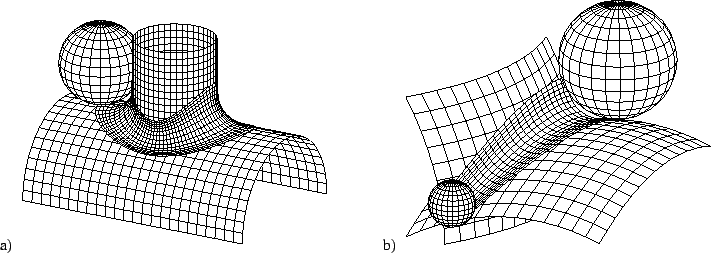
\includegraphics[width=\textwidth]{images/rolling_ball_blends.png}
	\caption[Technika rolling ball blends.]{Technika rolling ball blend s konštatným polomerom vľavo, s nekonštantným polomerom vpravo.}
	\label{fig:rolling_ball_blends}
\end{figure}
